\documentclass[10pt]{standalone}

\usepackage{pgfplots}
\pgfplotsset{compat=1.15}
\usepackage{mathrsfs}
\usetikzlibrary{arrows}
\pagestyle{empty}
\begin{document}

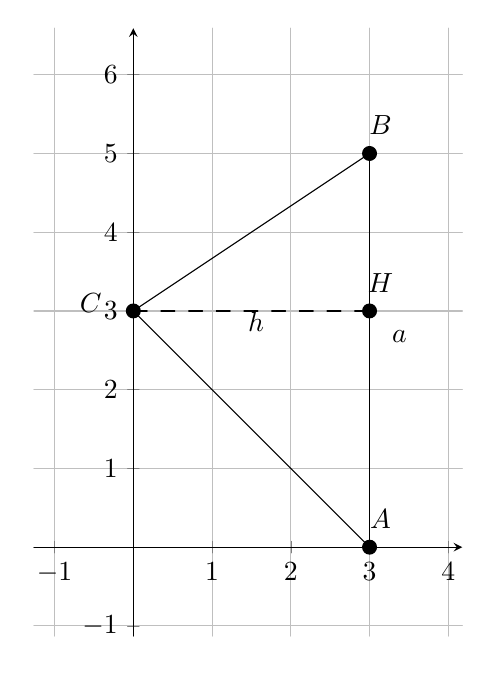
\begin{tikzpicture}[line cap=round,line join=round,>=triangle 45,x=1.0cm,y=1.0cm]
\begin{axis}[
x=1.0cm,y=1.0cm,
axis lines=middle,
ymajorgrids=true,
xmajorgrids=true,
xmin=-1.2614000000000019,
xmax=4.178599999999996,
ymin=-1.1293999999999997,
ymax=6.590600000000003,
xtick={-1.0,0.0,...,4.0},
ytick={-1.0,0.0,...,6.0},]
\clip(-1.2614,-1.1294) rectangle (4.1786,6.5906);
\draw  (3.,0.)-- (3.,5.);
\draw  (3.,5.)-- (0.,3.);
\draw  (0.,3.)-- (3.,0.);
\draw [dash pattern=on 5pt off 5pt] (0.,3.)-- (3.,3.);
\begin{scriptsize}
\draw [fill=black] (3.,0.) circle (2.5pt);
\draw[color=black] (3.1386,0.3606) node {$A$};
\draw [fill=black] (3.,5.) circle (2.5pt);
\draw[color=black] (3.1386,5.3606) node {$B$};
\draw [fill=black] (0.,3.) circle (2.5pt);
\draw[color=black] (-0.5414,3.1006) node {$C$};
\draw [fill=black] (3.,3.) circle (2.5pt);
\draw[color=black] (3.1386,3.3606) node {$H$};
\draw[color=black] (3.3786,2.6806) node {$a$};
\draw[color=black] (1.5586,2.8606) node {$h$};
\end{scriptsize}
\end{axis}
\end{tikzpicture}
\end{document}